\documentclass[main.tex]{subfiles}
\begin{document}

\chapter{Source foils design optimisation}


%\begin{flushright}
%\textit{The only thing that could save them was selenium.}\\
%Isaac Asimov, \textit{I, Robot, Runaround}.
%\end{flushright} 


\NI Over the years, many studies of the physics case of SuperNEMO with 82Se source were performed,  with the work found in [1] being the more complete and well documented.  The study conclude that in order to achieve sensitivity of $\sim$ 10$^{26}$ y in 500 kg $\times$ y of exposure with 82Se , the radio-purity level of the source foil in 208Tl and 214 Bi must be better than 2 $\mu$ Bq/kg and 10$\mu$Bq/kg respectively. Since  standard  HpGe  spectroscopy  is  not  sensitive  enough  to  such  low level of activities, the collaboration conceived and build the BiPo detector [2], with the specific purpose of measuring the radio-purity of the 82Se foils. The BiPo-3 detector is fully operative in LSC (Spain) since 2012 and the different components of the source foil are being measured. The challenging radio-purity requirement have triggered new R\&D work in order to explore alternative source foil design with respect to the design of the composite foil adopted in NEMO-3.  Two main design are currently under consideration: a NEMO-3-like foil made of 82Se , glue and two mylar backing film; a new design made of 82Se glue and a central nylon mesh. The different conception of the foils could, in principle, induce differences in the performance, e.g. in the background level and the sensitivity to the 0$\nu\beta\beta$ half-life. 


\bigskip


\NI Since [1] however the design of the detector has changed, being finalised for  the  construction  of  the  first  demonstrator  module.   Furthermore,  the recent  development  of  the  source  foil  design  and  the  results  of  the  first radio-purity measurement from BiPo motivate a more detailed study of the physics case of SuperNEMO. Chap.2 provides a detailed description of the different source foil design under consideration for the SuperNEMO demonstrator module. The recent results of the radio-purity measurement of the main foil components performed by BiPo are also shown. Chap.3 describes the software framework used to simulate events in the source foil, reconstruct the detector response and finally select events in the 2e hannel to obtain energy p.d.f. for signal and background. Chap.4 introduces two methods for the calculation of the sensitivity and compare among them.  A qualitative validation of the simulation used in this work is also performed in this chapter.  Finally, chap.5 provides a detailed study of the performance with respect to different design of the 82Se source foil.


\section{Source foil design}


\NI In the demonstrator phase, the source of double-beta decay is made of enriched 82 Se powder shaped in thin foils to minimise the energy loss of the out-coming particles and placed in the middle of the detector. To eliminate background events due to impurities in the source foil, the required radio-purity levels for 208 Tl and 214 Bi are very challenging. In order to shape the $\beta\beta$ emitter in thin foil, the 82 Se powder is mixed with a polyvinyl-alcohol (PVA) glue to produce a solid and uniform thin foil. A mechanical support is required to provide enough strength over 3 m long foil. Different material can be considered as mechanical support for the foil as well as different amount of PVA could be used. However the choice of the best materials and the design of the foil must be performed taking into account different aspect :


\begin{itemize}
\item radio-purity level in Tl208 and Bi214
\item Mass of a given material w.r.t Se82 mass
\item thickness of the foil
\end{itemize}


\NI The best design and the optimal composition of the foil will depend from the performance we could obtain by installing such a foil in the SuperNEMO demonstrator module. We already know that an IDEAL foil composed only of 82 Se would allow to obtain the best performance, but given the chemical characteristics of the selenium, this is unfortunately very hard, perhaps unfeasible. For this reason the collaboration is currently considering two main designs, here after named MYLAR and TULLE. In the following sections the different materials under consideration for the foil production and their levels of radio-purity, as measured by the BiPo detector, will be discussed. The detailed description of the foil designs under consideration is provided, including the IDEAL design which can be used as a reference or best-case-scenario for comparisons.


\subsection{Foil composition}


\NI The materials under consideration for the thin foil production are described in the following lists:


\begin{itemize}


\item \textbf{Selenium} : A nonmetal with properties that are intermediate between those of its periodic table column-adjacent chalcogen elements sulphur and tellurium. It rarely occurs in its elemental state in nature, or as pure ore compounds. Selenium salts are toxic in large amounts, but trace amounts are necessary for cellular function in many organisms, including all animals. As prepared in chemical reactions, selenium is usually amorphous, brick-red powder. When rapidly melted, it forms the black, vitreous form, which is usually sold industrially as beads. The structure of black selenium is irregular and complex and consists of polymeric rings with up to 1000 atoms per ring. Black selenium is a brittle, lustrous solid that is slightly soluble in CS 2 . Selenium has six naturally occurring isotopes, five of which are stable: 74 Se, 76 Se,77 Se, 78 Se, and 80 Se. The final naturally occurring isotope is the 82 Se which decay via double beta decay to 82 Kr with very long half-life of 9 $\times$ 10 19 y, as measured by NEMO3 experiment [3].


\item \textbf{Polyvinyl alcohol} : Polyvinyl alcohol (PVOH, PVA, or PVAl) is a water-soluble synthetic polymer (not to be confused with polyvinyl acetate, a popular wood glue). It has the idealised formula [CH 2 CH(OH)] n . It is used in paper-making, textiles, and a variety of coatings. It is white (colourless) and odourless. It is sometimes supplied as beads or as solutions in water.


\item \textbf{Mylar} : BoPET (Biaxially-oriented polyethylene terephthalate) is a polyester film made from stretched polyethylene terephthalate (PET) and is used for its high tensile strength, chemical and dimensional stabil- ity, transparency, reflectivity, gas and aroma barrier properties, and electrical insulation.


\item \textbf{Nylon6-6} : Polyamide from nylon class, made of hexamethylenediamine and adipic acid, which give nylon 6-6 a total of 12 carbon atoms in each repeating unit, and its name. Nylon 6-6 is frequently used when high mechanical strength, great rigidity, and good stability under heat is required.


\end{itemize}


\subsection{Material radio-purity}


\NI The level of contamination in 208 Tl and 214 Bi of the materials under consideration for the foil production have been measured in BiPo [4]. The activities in 208 Tl and 214 Bi at 90\% C.L. are summarised in Tab. 2.1. Those 6 values are used in the following to estimate the background contaminating the search for 0$\nu\beta\beta$ event in the SuperNEMO demonstrator module.


\subsection{Foil geometry}


\NI The foil geometry is shown in fig. 2.1. It consist of 36 strips 2700 cm long for a total surface of about 14 m 2 which will contain 7 kg of 82 Se , with a surface density of about 50 mg/cm 2 . While the total mass of 82 Se is already known, the amount of the other components will depend of the foil design and it is the subject of this study.


\subsection{Foil parameters}


\NI Before entering in the details of the different foil designs, it is useful to define some parameters which allow to characterise different foil compositions. When mixing two or more materials in order to obtain an uniform compound it is important to know the mass fraction f i of a given component, defined as the ratio of its mass M i with respect to the total mass of the compound M T :


\bigskip	


\NI The density of the compound is then defined as the mean of the density of each ingredient properly weighted on their mass fraction :


\bigskip


\NI In the case such uniform compound is used to produce a foil, i.e. it is uniformly spread over a flat surface S, it is also useful to define the foil surface density as :


\bigskip


\NI and the thickness of the foil as :


\bigskip


\NI As shown by 2.4 the thickness of the foil increase linearly with the mass of the components but decrease linearly with the total density of the compound. An important parameters to characterise the radio-purity foil design is the total expected activity in 208 Tl and 214 Bi . Given the activities measured by BiPo and summarised in 2.1, the total activity of the foil is usually expressed in term of the total mass of 82 Se :


\subsection{Designs under consideration}


\NI The main design of the source foil being considered for the SuperNEMO demonstrator module are described in the following.


\subsubsection{IDEAL}


\NI The IDEAL foil design represent a source foil made of 82 Se mixed with a small fraction PVA (< 5\%) to glue the 82 Se powder grain. This design must be considered an ideal case since, from the technical point of view, it is be very hard to produce. Furthermore, a 2.7 m long foil made of only from 82 Se and PVA will be too fragile to be handled and installed in the SuperNEMO source frame. The IDEAL design is nonetheless interesting since it represents the simpler design we could consider at this stage. Compared to more realistic design, the absence of a mechanical support and the small amount of PVA would provide a thinner foil with smaller contamination in 208 Tl and 214 Bi and as a consequence a smaller level of background.


\subsubsection{MYLAR}


\NI The MYLAR design is based on the experience developed in NEMO3. The 82 Se + PVA paste at about 5\% is spread as uniform as possible within two mylar films. The mylar films are exposed to an ion beam to produce micro holes which allow the water present in the paste to evaporate and dry the foil. The film has a thickness of 12 $\mu$m and a mass of about 2.5 mg/cm 2 . A schematic view of the foil design is shown in fig. 2.2. The mylar acts as backing film for the 82 Se source foil, providing mechanical support all over the 2.7 m length and protecting against losses of 82 Se powder. It must be noticed that the backing film will provide additional contamination with respect to the IDEAL case.


\subsubsection{TULLE}


\NI This is a new conception of the source foils. The 82 Se + PVA paste is spread as uniform as possible over a thin layer of bobbinet tulle made of nylon6-6 which provides a light but resistant mechanical support. A schematic view of the foil design is shown in fig. 2.3. The bobbinet tulle is constructed by warp and weft yarns in which the weft yarn is looped diagonally around the vertical warp yarn to form a hexagonal mesh which is regular and clearly defined. Bobbinet netting has a characteristic diagonal fabric appearance, is diagonally stable and slide-proof, durable, sheer and has a high strength to weight ratio.In order to minimise the contamination in 208 Tl and 214 Bi coming from the tulle, the lightest fabric available on the market has been chosen, corresponding to a weight of 0.7 mg/cm 2 . To our request, the batch of tulle we obtain was not treated with resins nor paint after waving. Given the lightness of the tulle sheet with respect to the mylar backing film, this design has the advantage to introduce a smaller contamination of 208 Tl and 214 Bi which will translate in lower background levels. On the other hand, the lack of an external protection sheet exposes the foil to the risk of 82 Se losses. This problem could be reduced by increasing the amount of PVA glue mixed with the 82 Se in order to increase the foil strength. An increase of the foil mass induce an increase of the contamination, nonetheless the choice of a lighter mechanical support will compensate the increase of PVA. Laboratory tests suggest that a TULLE foil design containing 10\% of PVA will be resistant enough and this composition is used as baseline in the following. This value will be validated and optimised by studying the detector performance in chap. 5.


\subsection{Discussion}


\NI The source foil design under consideration for the SuperNEMO demonstrator has been introduced. Tab. 2.2 and tab. 2.3 summarise the design parameters to consider when modelling the foils in the simulation code. The MYLAR foil is considered as an IDEAL foil with two external backing films, the parameters in this case are shown separately for the bulk (b) and the film (f). The TULLE foil is modelled as an IDEAL foil with the nylon mesh uniformly distributed in the foil.


\bigskip


\NI As shown in tab. 2.3 the TULLE design is very promising from the radio- purity point of view. Even if this design require more PVA to glue the 82 Se powder together, the lightness of the tulle support and its low contamination allow to obtain a total activity in 214 Bi and 208 Tl which is respectively 18\% and 29\% lower than what it is expected for the MYLAR design.


\section{Monte-Carlo simulations}


\NI The study performed in this work is based on the event simulation performed through the Falaise-legacy framework. Through a set of configuration files, the user can specify the detector model to be considered (i.e. geometry and materials) and simulate the initial kinematic for different type of events in specific region of the detector (e.g. the source foil). The propaga- tion of the particles through the detector is performed by a GEANT4 based module which simulates all relevant processes, such as multiple scattering, ionisation, Compton scattering, bremsstrahlung. The detector response is then obtained by smearing the true information provided by GEANT4 with respect to the calorimeter and the tracker resolution. Dedicated reconstruction and selection module allow to select events in a specific channel for dedicated analysis.


\bigskip


\NI This work is not meant to document and validate the Falaise-legacy chain, a complete validation of the framework should be found elsewhere. The description available in the following focuses only on the parts relevant for this work. Moreover, the Falaise-legacy is likely to be abandoned in favour of a new version of the framework which is currently under validation. The new software should be used in the future to cross-check the MC production used for this work.


\subsection{Source foils modelisation}


\NI In the simulation code, the source foil strips shown in fig. 2.1 are modelled through rectangular boxes made of 82 Se , PVA glue, nylon or mylar depending from the design being considered. The detailed composition of the different design has already been discussed in sec. 2.5 and the parameters to be considered are summarised in tab. 2.2. The implementation of the material composition is performed by defining the fraction mass for each element, mainly 82 Se , Nat Se, O, C and N which is found in the nylon mesh.


\subsection{Events generation}


\NI Events generated uniformly from the source foil are considered. A part from
the 0$\nu\beta\beta$ and the irreducible 2$\nu\beta\beta$ background, the internal background coming from contamination in 208 Tl and 214 Bi are also considered. Since the geometric model of the MYLAR design account for the two mylar layers surrounding the bulk made of 82 Se and PVA, 208 Tl and 214 Bi are generated both in the bulk and in the mylar film in order to account for contamination coming from the mylar with the correct p.d.f. The values in tab. 3.1 show the statistics generated for each event type.


\bigskip


\NI Since the event generation has been performed with many different configurations of the source foil, the statistics has been optimised to contain the event production within reasonable processing time (∼24 hours). As will be shown later, the current production allows to keep the statistical uncertainty on the number of events selected in the relevant energy region within ∼0.2\% for the 0$\nu\beta\beta$ and the 2$\nu\beta\beta$ events and within ∼5\% for the 208 Tl and 214 Bi events. The statistical uncertainties on the 208 Tl and the 214 Bi are rather high for a typical MC study. Despite they could be reduced generating more events, they are already a factor 2 lower than the systematic uncertainties observed for the internal background in NEMO-3 (10\%) . In SuperNEMO, these systematics are expected to remain of the same order of magnitude, so the 5\% statistical uncertainty on the MC samples is enough in this contest.


\subsection{Events energy distribution}


\NI The reconstructed events are selected in the 2e channel through a simple selection criteria which requires two negative tracks hitting two calorimeter blocks with a total energy deposition E $\beta\beta$ > 2 MeV. The signal and background energy p.d.f.s are shown in fig. 3.1. The shape of the energy distribution does not depend strongly on the design under consideration, while there is an overall decrease of the event selection efficiency for the TULLE and the MYLAR designs w.r.t. the IDEAL case. The values in tab. 3.2 shown the event selection efficiencies for the signal and the background obtained in the [2000; 3200] keV energy window. The decrease is more important for the 0$\nu\beta\beta$ and 2$\nu\beta\beta$ while it is not significant for the 208 Tl and the 214 Bi. The effect is due to the increased thickness of the source foil in the TULLE and the MYLAR designs w.r.t. to the IDEAL case, which slightly shifts the p.d.f. to the lower energies due to an increased energy loss in the foil.


\subsection{Conclusion}


\NI The relevant informations to obtain the signal and background p.d.f. in the 2e channel have been summarised. The p.d.f. will be used in the following chapters to compare among different designs of the source foil. As already mentioned, a full validation of the Falaise-legacy framework has not been performed here. A qualitative validation of the framework with respect to the results reported in [1] and [6] will be provided in the next chapter.


\bigskip


\NI However, the optimisation of the source foil design does not require an absolute validation of the simulation code. As far as the results are compared in a relative way among the different design being considered, the conclusion will remain valid, even in case of bugs in the software. The Falaise legacy pipeline configuration files, the geometry model of the source foil designs as well as a set of scripts to automatise the job submission at ccin2p3 have been organised in a package called foil study legacy. The package is available from the lpc caen svn repository , the tag v1.0.0 is the recommended release to reproduce the results obtained in this note.


\section{Sensitivity study}


\NI The study of the sensitivity of an experiment looking for a new phenomena, allows to estimate its physics case and compare among different competing experiments. During the designing phase, it is also useful to study the sensitivity with respect to different detector configurations in order to find the optimal design.


\bigskip


\NI In order to define the sensitivity to a phenomena not yet observed, we assume the experiment does not observe any signal. In this worse case scenario, we study which portion of the allowed parameter phase space the experiment can exclude.


\bigskip


\NI In the following sections, different methods to compute SuperNEMO sensitivity are described in details. The sens software package, which implements each sensitivity computation method, is also described. This section serves as reference manual for the user. The p.d.fs obtained in the previous chapter with the IDEAL design are used in the following as example of sensitivity computation. Here the backgrounds are normalised to 2 $\mu$Bq/kg and 10 $\mu$Bq/kg for the 208 Tl and the 214 Bi internal background respectively (i.e. the target radio-purity level of SuperNEMO). The 2$\nu\beta\beta$ background is normalised to 9 $\times$ 10 19 y as measured in NEMO-3 [7]. This configuration is referred in the text as IDEAL (star).



\subsection{R.O.I method}


\NI The sensitivity of a 0$\nu\beta\beta$ experimental search is defined as a limit on the decay half-life :


\bigskip


\NI where N A is the Avogadro number, W the atomic mass of the $\beta\beta$ isotope under study, the signal selection efficiency and M $\times$ T the total experimental exposure. The term S(b) represents the average upper limit on the number of signal events that would be obtained by an ensemble of identical replicas of such experiment, each one with the same mean expected background and no true signal. The Feldman \& Cousins unified approach for the definition of the confidence level is adopted.


\bigskip


\NI This method optimise the R.O.I. with respect to the sensitivity to the T 1/2
Such optimisation is achieved by maximising th $\epsilon$/S(b) ratio for a given exposure M $\times$ T.


\subsection{Selection efficiency}


\NI The signal and the background selection efficiencies in the 2e channel are obtained integrating the respective p.d.f.


\bigskip 


\NI Where the energy interval (E Low ; E Up ) define the R.O.I.. The plot in fig. 4.1 show the value of efficiency for the 0$\nu\beta\beta$ signal (red) and background (2$\nu\beta\beta$ in blue, 214 Bi in yellow and 208 Tl in green) when the upper edge of the R.O.I. is kept fix at 4500 keV while the lower edge is moved from 2000 keV up to 3500 keV.


\bigskip


\NI Those efficiencies are then used to estimate the expected background level for a given exposure M $\times$ T following :


\bigskip


\NI Where T 1/2 Is the measured half-life for the 2$\nu\beta\beta$ decay while A214Bi and 208 A 208Tl are the expected activity level of Bi and Tl contamination of the foil source. The renormalisation of the histogram in fig. 4.1 through eq. 4.3, 4.4 and 4.5 provide the expected number of background events as a function of the low energy edge of the R.O.I. as shown in fig. 4.2.


\bigskip


\NI The integral of eq. 4.2 can also be computed changing both edges of the R.O.I. obtaining a 2D scan of the selection efficiencies. The same renormalisation through eq. 4.3, 4.4 and 4.5 provide the 2D scan of the expected number of background events w.r.t. the edges of the R.O.I. as shown in fig. 4.3.


\subsection{The Feldman \& Cousins 90\% C.L.}
 

\NI The term S(b) of eq. 4.1 is defined following the Feldman \& Cousins prescription for the definition of confidence interval of small signal [8]. Defining U(n$|$b) as the function yielding the (unified approach) upper limit (at the desired C.L.) for a given observation n and a mean predicted background level b. Values for U(n$|$b) are reported in tabular form in [?] for several C.L. values. Given that the variable n follows a Poisson p.d.f., P(n$|$b) = P(n; b), then S(b) is given by : 


\bigskip


\NI The sensitivity S(b) of an experiment expecting b events of background and no true signal is obtained by averaging the upper limits obtained using the unified approach U(n$|$b) with the likelihood of the individual observations P(n$|$b). The fig. 4.4 shows the 90\% C.L. curve for a background level spanning in [0; 40] c.t.s. It must be noticed that in the large background approximation, the sensitivity curve as a function of b follows the expected classical limit obtained through the Neyman construction of the confidence belt :


\bigskip


\NI where a =1.64 (1.96) at 90\% (95\%) CL.


\subsection{1d vs 2d R.O.I. optimisation}


\NI Computing the sensitivity from eq. 4.1 as a function of the R.O.I. for a given experimental exposure define the best sensitivity of the experiment. The plot in fig. 4.5 show the 1d sensitivity scan as a function of the low energy edge of the R.O.I.. The high energy edge is kept fix at 3200 keV. The best sensitivity of 6.1$\times$10 24 y is found in [2720; 3200] keV after 21 kg$\times$y exposure, with an expected total background contamination of 0.74 $\pm$ 0.06 cts. in the R.O.I..


\bigskip

\NI Since the decay chain of the 208 Tl has an high energy gamma, the expected 2e energy spectral shape extend at high energy up to 3500 keV, above the end point of the $\beta\beta$ energy spectrum of the 82 Se at Q $\beta\beta$ = 2995 keV as shown in fig. 4.2. In order to minimise such background contamination, the simultaneous optimisation of the two edges of the R.O.I. is performed in fig. 4.6. The best sensitivity of 6.12 $\times$ 10 24 y is found in [2720; 3060] keV after 21 kg$\times$y exposure, with an expected total background contamination of 0.72 $\pm$ 0.06 cts. in the R.O.I.. No major reduction of the background is observed, the results are found to be compatible within the statistical uncertainties.


\subsection{Validation of the background level}


\NI As already mentioned, the results of the simulation performed with the Falaise-legacy framework has not been validated in details here. The recent NEMO-3 results on the 100 Mo [6] could be used to crosscheck the background level obtained in sec. 4.1. The eq. 4.3, 4.4 and 4.5 could in fact be used to scale the background measured in NEMO-3 to the target 208 Tl and 214 Bi activities and to the exposure of the SuperNEMO demonstrator.


\bigskip


\NI The values in tab. 4.1 shown the internal 208 Tl and 214 Bi activities measured in NEMO-3, the measured background level in [2.8; 3.2] MeV and its extrapolation to the activities and exposure expected for the SuperNEMO demonstrator. The last column of the table shows the expected background level extracted from fig. 4.3, considering the same R.O.I. as NEMO-3. 


\bigskip


\NI A discrepancies of 33\% and 42\% is observed for the 208 Tl and the 214 Bi respectively. However, it must be kept in mind that a direct comparisons could not apply since NEMO-3 and SuperNEMO are not the same detector. SuperNEMO in fact has a better energy resolution (8\% at 1 MeV w.r.t. the 14\% of NEMO-3) and an higher detection efficiency due to an optimised design of the tracker and the calorimeter. While NEMO-3 has a 0$\nu\beta\beta$ detection efficiency of 4.7\% in [2.8; 3.2] MeV, for SuperNEMO this value is 11\%, as obtained from the simulation performed in this work. Neglecting the different energy resolution (208 Tl and 214 Bi spectra are rather flat in the R.O.I.) the values of tab. 4.1 agrees within 20\% when considering that the 0$\nu\beta\beta$ selection efficiency of SuperNEMO is $\times$ 2.3 higher than NEMO-3.


\subsection{Validation of the sensitivity calculation}


\NI The sensitivity value obtained with the extended likelihood method in sec. 4.2 could be compared to the results obtained in [1], since the method is the same. The plot in fig. 4.8 shown the T 1/2 an exposure of 500 kg$\times$y as a function of the calorimeter energy resolution obtained in [1]. The dependence of the thickness of the source foil is also shown with different colour. The internal background activities have been set to 2 $\mu$Bq/kg and 10 $\mu$Bq/kg for 208 Tl and 214 Bi respectively.


\bigskip


\NI Even if the design of the detector adopted in [1] is slightly different to the final one being considered in this work, a qualitative comparisons could be performed choosing the values corresponding to the current detector parameters. The final detector design adopted in this work consider a calorimeter resolution of 8\% FWHM at 1 MeV and a source foil thickness of 50 mg/cm 2 . The relevant sensitivity value from fig. 4.8 is then between 7.5 $\times$ 10 25 y and 9.5 $\times$ 10 25 y corresponding to a thickness of 40 mg/cm 2 and 60 mg/cm 2 respectively.


\bigskip


\NI The extrapolation of the calculation performed in the previous section up to 500 kg$\times$y results in a sensitivity of 8.3 $\times$ 10 25 y at 90\% C.L which agrees within 12\% with the values obtained in [1]. The agreements improve to 3.5\% when the 208 Tl and 214 Bi internal backgrounds are neglected.


\subsection{Estimation of the systematic uncertainty}


\NI The uncertainty on the sensitivity calculation could be roughly estimated assuming the same systematic uncertainties as NEMO-3. The results obtained in [6] quote the following uncertainties in the R.O.I.: $\pm$10\% on the 0$\nu\beta\beta$ selection efficiency $\pm$ 0.7\% on the 2$\nu\beta\beta$ background and $\pm$10\% for both 214 Bi and 208 Tl background. Taking into account those values in the sensitivity calculation with the R.O.I. method, an uncertainty of about $\pm$11\% is obtained on the half-life limit. The worse case scenario in which the signal selection efficiency and the backgrounds fluctuate in opposite directions is assumed for simplicity. The tab. 4.2 summarises the results of the sensitivity scan taking into account the NEMO-3 systematics uncertainties.


\section{Source foil design and detector performance}


\NI The event simulated through the Falaise-legacy software and the method developed in chap.4 to compute the sensitivity are used in the following sections to study the performance of the SuperNEMO detector. The background level and the sensitivity achievable with the different designs of the source foil introduced in chap. 2 are compared in sec. 5.1 and 5.2 respectively. The amount of PVA glue to mix with 82 Se during the production of the TULLE design is optimised in order to provide competitive performance with respect to the alternative MYLAR design in sec. 5.3. Finally the effects of a non uniform thickness of the source foil is evaluated in sec 5.4 providing a target value for the foil production.


\subsection{Radio-purity vs background level}


\NI The different designs of the source foil have an impact on the event selection efficiency in the 2e channel, as highlighted in tab. 3.2 considering events in the [2000; 3200] keV energy region. These differences translate into a different background level for a given internal contamination and a given exposure. Assuming an exposure of 21 kg$\times$y the expected level of background in the optimised R.O.I. is computed changing the 208 Tl and the 214 Bi activity from 0 $\mu$Bq/kg to 15 $\mu$Bq/kg. The resulting histograms are shown in fig. 5.1. The fig. 5.2 shows the amount of internal contamination only, i.e. without the contribution from 0$\nu\beta\beta$ events. It should be noted that for the MYLAR design, each value of activity is equally shared among the p.d.f. of the bulk and the backing film. If all the activity is given to the bulk p.d.f. only, the background increase by 10 . Compatible background level is found as a function of the 208 Tl and 214 Bi activities among the source foil designs. At the target radio-purity level of 2 $\mu$Bq/kg in 208 Tl and 10 $\mu$Bq/kg in 214 Bi the expected background coming from the internal contamination is 0.15 counts for an exposure of 21 kg$\times$y.


\subsection{Sensitivity vs. foil designs}


\NI The values in tab. 5.1 summarise the performance achievable with the SuperNEMO demonstrator module with respect to the source foil design, considering an exposure of 21 kg$\times$y. The signal and the background p.d.f. obtained as described in chap. 3 has been normalised to the 208 Tl and 214 Bi activities measured by BiPo and summarised in tab. 2.3. The label IDEAL star in tab. 5.1 refers, as in chap. 4, to IDEAL design case in which the background p.d.f. are normalised to the target radio-purity level of SuperNEMO. The plots in fig. 5.3 show the result of the sensitivity scan w.r.t. the energy edges of the R.O.I.


\bigskip


\NI As discussed in sec. 3.3, the design of the source foil does not have a strong impact on the shape of the signal and background energy distributions. Nonetheless, the different activities of the material considered for the foil production and their mass fraction with respect to the 82 Se affect in a non negligible way the performance of SuperNEMO. With respect to the IDEAL design, the performance decreases by about 16\% for the TULLE design and about 16\% for the MYLAR design. The TULLE and the MYLAR design are compatible within 3\%. The plot in fig. 5.4 shows the extrapolation of the SuperNEMO sensitivity beyond the exposure expected for the demonstrator module, up to 1000 kg$\times$y.


\bigskip


\NI The comparison performed so far neglects the residual contamination of 208 Tl and 214 Bi expected in the 82 Se powder, since any value is available at present. Since no major improvement has been obtained, or proven, in the 82 Se purification process so far, the 82 Se contamination could be the dominant contribution to the background, regardless the design of the source foil. In tab. 5.2 the performance of SuperNEMO has been studied considering an additional contamination of 100 $\mu$Bq/kg both in 208 Tl and 214 Bi, as it could be expected from the 82 Se . The overall effect is a reduction of the discrepancies observed among the source foil design down to 11\% and 13\% for the TULLE and the MYLAR respectively. A high contamination of the 82 Se would then make the choice of the source foil design rather equivalent. This study will be updated as soon as the radio-purity measurement of the 82 Se powder will be available.



\subsection{Optimising the amount of PVA}


\NI In this section the optimal amount of PVA to mix with 82 Se during the production of the TULLE design is optimised in order to provide compatible performance with respect to the alternative MYLAR design. As shown in tab. 5.3, the variation of the amount of glue impact the thickness of the foil, i.e. the shape of the signal and background p.d.f. as shown in fig. 5.5, as well as the background level. The values in tab. 5.4 summarise the results of the performance study as a function of the amount of glue.


\bigskip


\NI Even if the best performances are obtained without glue, such scenario is not technically feasible since the 82 Se foil will not be resistant enough. A TULLE foil containing 5\% of PVA would still be compatible to the IDEAL design within 10\%, but it would be very hard to produce it, as observed during the R\&D tests at LAPP. From the technical point of view, a fraction of 10-15\% of PVA seems more reasonable and would allow to achieve performance compatible to the MYLAR design within 10\%.


\subsection{Foil uniformity}


\NI The thickness of the source foil impact the energy losses of the out-coming particles worsening the resolution on the energy measurement. For similar reasons, the thickness impacts also the probability of observing 2e events from the beta decay of 208 Tl and 214 Bi . During the production of the source foil, the 82 Se + PVA paste is poured on a dedicated support and spread uniformly over the surface. Since the process is performed manually, a non uniform deposition of the paste may happen. This will cause a non uniform thickness over the foil length affecting the performance of the SuperNEMO demonstrator in terms of background level and sensitivity. For this reason is important to study such effects in order to define the acceptable level of uniformity of the source foil.


\subsubsection{Signal and background vs foil thickness}


\NI Signal and background events has been simulated considering a TULLE foil design containing 90\% of 82 Se and 10\% of PVA. The reference thickness of 190 $\mu$m has been varied by $\pm$10\% and $\pm$20\%. For each foil thickness, the simulated sample consists of 10 6 0$\nu\beta\beta$ events and 10 7 events for each background channel, 2$\nu\beta\beta$ , 208 Tl and 214 Bi . The expected energy spectra of the 2e  channel are shown in fig. 5.6 for the different thicknesses. It appear clearly looking at the 0$\nu\beta\beta$ (top left) and the 2$\nu\beta\beta$ top right) spectra of fig. 5.6 that the overall effect is a worsening of the energy resolution (increasing of the 0$\nu\beta\beta$ peak width) and a shift of the events toward lower energies due to a increase of the energy lost within the foil. Tab. 5.5 summarises the impact of the source foil thickness on the selection efficiency for the signal and the backgrounds. The selection efficiency being defined as the fraction of events satisfying the simple selection criteria of two reconstructed negative tracks hitting two calo blocks with a total energy deposition E $\beta\beta$ > 2 MeV. Uncertainties on the efficiencies are statistical only. Tab. 5.6 shows the same observables obtained for E $\beta\beta$ in 0$\nu$ . [2700; 3000] MeV, defined as the ROI maximising the sensitivity to T 1/2 The total background level and the best sensitivity obtained in the ROI are summarised in Tab. 5.7.


\subsubsection{Effects of the foil uniformity}


\NI To mimic the effect of a non uniform foil thickness, we consider a case in which half of the foil is, for example, +10\% thicker and the other half is -10\% thinner than the nominal value. The average thickness of such a foil is still the nominal value and the amount of 82 Se + PVA paste required to produce it would be unchanged. The overall effect of such a non uniformity on a generic observable x is then obtained by averaging the same observable x + and x - obtained for the thicker and the thinner foil respectively. The relative comparison against the same observable obtained with the nominal thickness allows to obtain the systematic effect $\sigma$ due to the non uniformity:


\bigskip


\NI The red and the blue histograms in fig. 5.7 show the averaged spectra obtained varying the foil thickness by $\pm$10\% and $\pm$20\% respectively. The black histogram shows the expected spectra at the nominal thickness of 190 $\mu$m. Tab. 5.8 shows the systematic effects on the signal and background selection efficiencies induced by a foil non uniformity for E $\beta\beta$ in [2000; 3100] keV. The effect of a variation of the foil thickness by $\pm$20\% is 0.5\% for the 0$\nu\beta\beta$ while it is slightly higher for the background events, remaining however within the statistical uncertainty of the simulated samples of about 5\%.


\bigskip


\NI Tab. 5.9 shows the effects in [2700; 3000] keV, where the best sensitivity is found. The effect of the thickness uniformity on the 0$\nu\beta\beta$ sample is < 3\% while for 2$\nu\beta\beta$ it increases up to 6\%. For the other internal background, the effect is < 8\%. The overall effect on the sensitivity is < 3\%. Assuming the systematic uncertainty on the signal and background efficiencies of 7\% and 10\% respectively [6] as the upper limit for the SuperNEMO demonstrator module, it is recommendable to aim for an uniformity <20\% over the whole foil surface. The effect of a $\pm$20\% uniformity remains in fact within the expected systematic uncertainties. In any case, it must be kept into account that the uniformity effects highlighted in this work could be reduced and perhaps neglected through a precise knowledge of the foil average thickness and a thickness map. Such a knowledge could be easily obtained through a dedicated measurement campaign (5\% at 200 $\mu$m) and then introduced in the geometry model of the SuperNEMO simulation software.


\section{Conclusion}


\NI The sensitivity of the SuperNEMO detector to the 0$\nu\beta\beta$ decay of 82 Se has been studied for different source foil designs. The different characteristics of the foils under consideration have been introduced with detail in chap. 2. The performance achievable with the TULLE and the MYLAR designs are compared to the IDEAL case in which the foil does not have any mechanical support. The event simulation and the recipe for the sensitivity calculation have been introduced in chap. 3 and chap. 4 respectively. The Falaise legacy software used in this work for the event simulation has not been fully validated here. A qualitative comparison with older studies shows however that the results are compatible. Anyway, the optimisation of the source foil design does not require an absolute validation of the simulation code as far as a relative comparison among the different designs is considered. Finally, in chap. 5 the performance of the SuperNEMO demonstrator module is studied. The design of the source foil does not have a strong impact on the shape of the energy distributions within the statistical uncertainties of the generated samples, 0.2\% and 5\% for signal and background respectively. Nonetheless, the different activities of 208 Tl and 214 Bi in the materials considered for the foil production and their mass fraction with respect to the 82 Se affect in a non negligible way the performance of SuperNEMO. With respect to the IDEAL design, the performance decreases by about 17\% and 22\% for the TULLE and the MYLAR design respectively. The TULLE and the MYLAR designs are compatible within 3\% among them. The differences among the designs decrease as the activities in 208 Tl and 214 Bi increase, making the choice of the source foil design rather equivalent in case of an high contamination coming, for example, from the 82 Se . The effect of a non uniformity on the thickness of the source foil has also been studied. The result of the sensitivity calculation performed for different thicknesses of the foil recommends an uniformity <20\% over the whole foil surface.



\begin{figure}[h!]
\centering
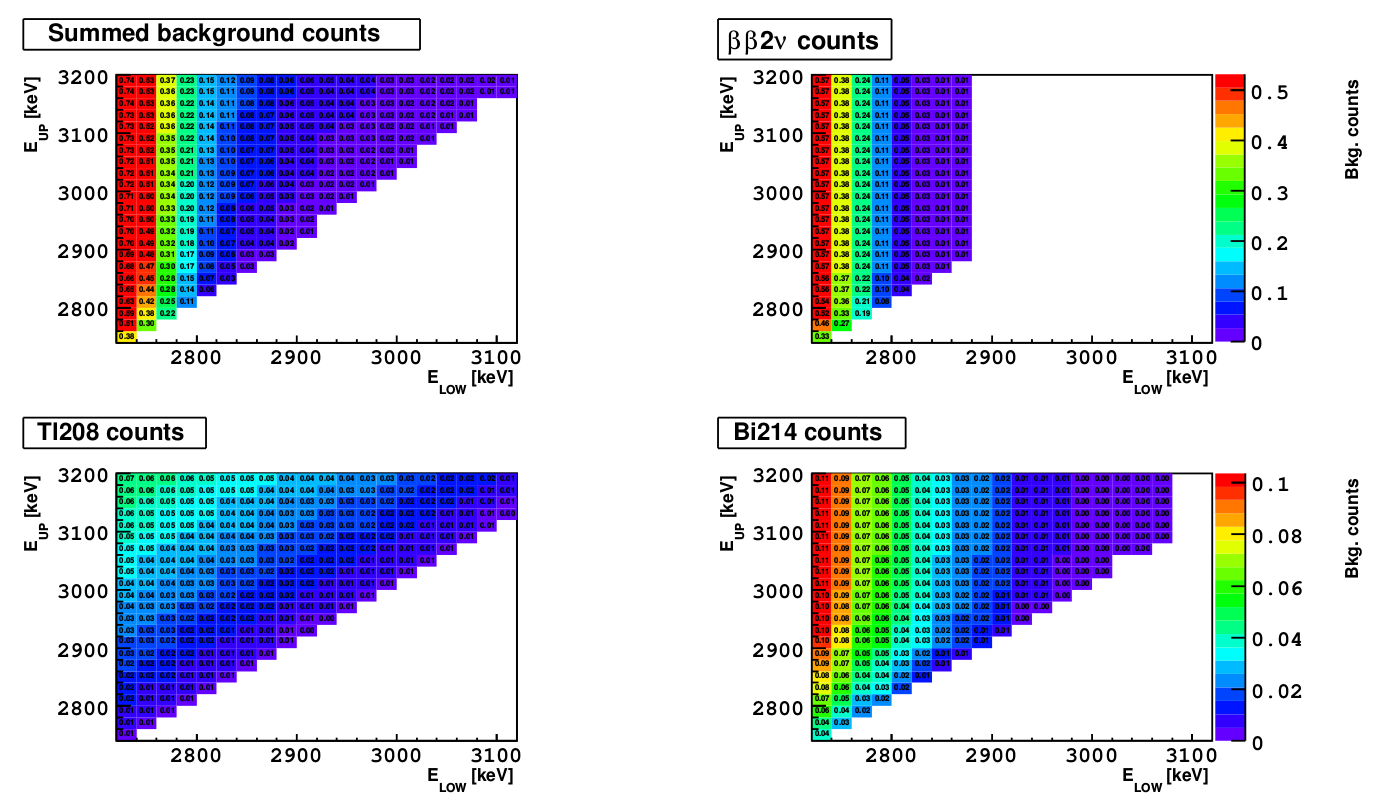
\includegraphics[scale=0.3]{pictures/Chap4/BkgCount2D.png}
\label{BkgCount2D.png}
\caption{aaa}
\end{figure}


\begin{figure}[h!]
\centering
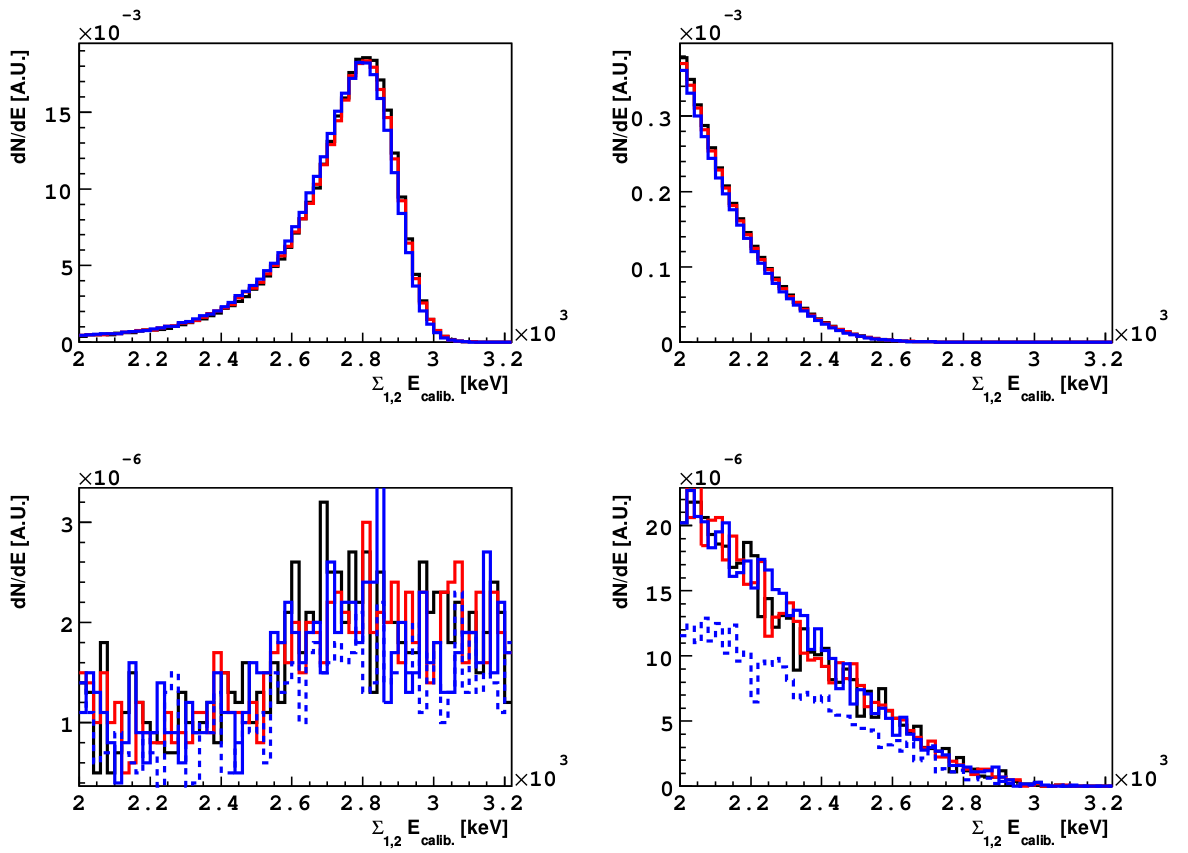
\includegraphics[scale=0.3]{pictures/Chap4/Distribution2eSelection.png}
\label{Distribution2eSelection.png}
\caption{aaa}
\end{figure}


\begin{figure}[h!]
\centering
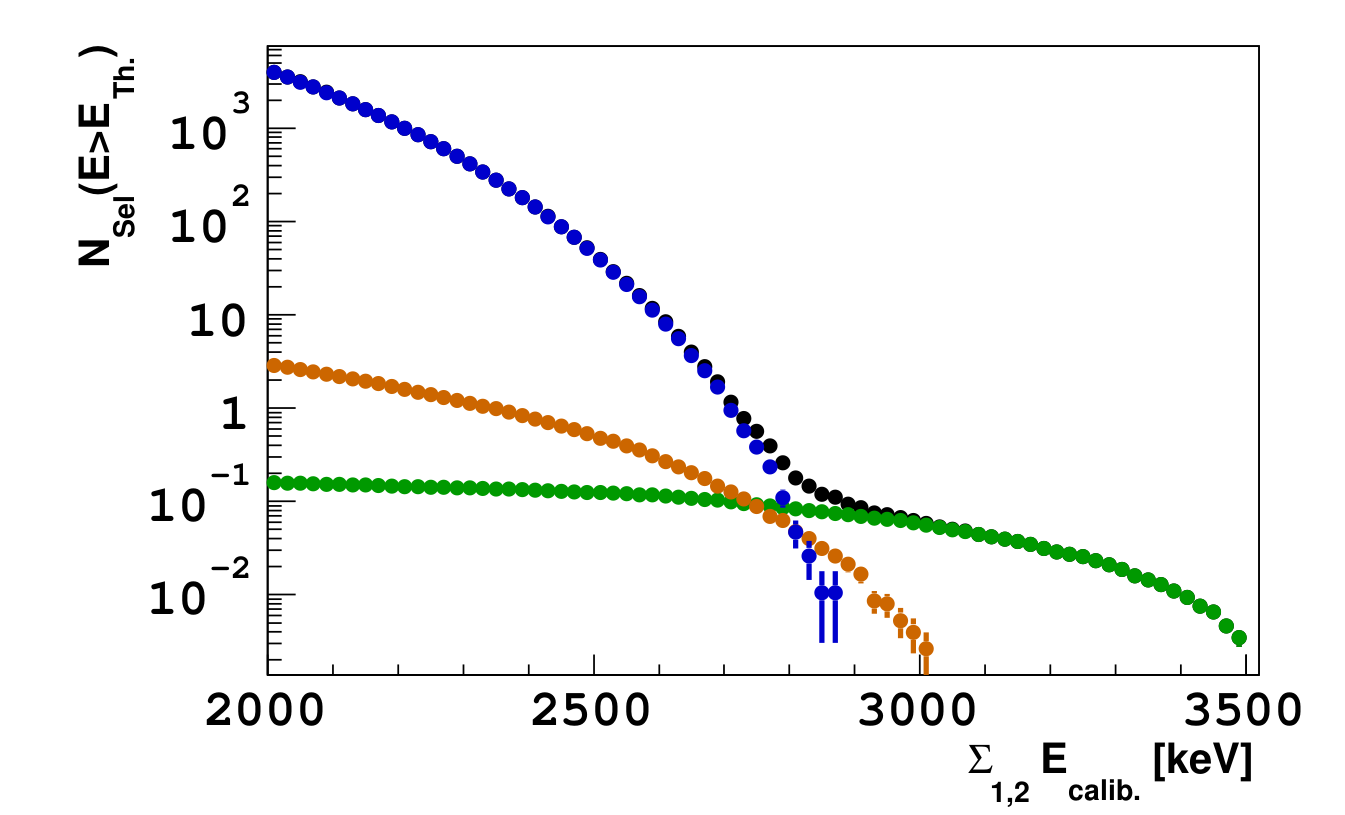
\includegraphics[scale=0.3]{pictures/Chap4/ExpectedNumberofEvent.png}
\label{ExpectedNumberofEvent.png}
\caption{aaa}
\end{figure}


\begin{figure}[h!]
\centering
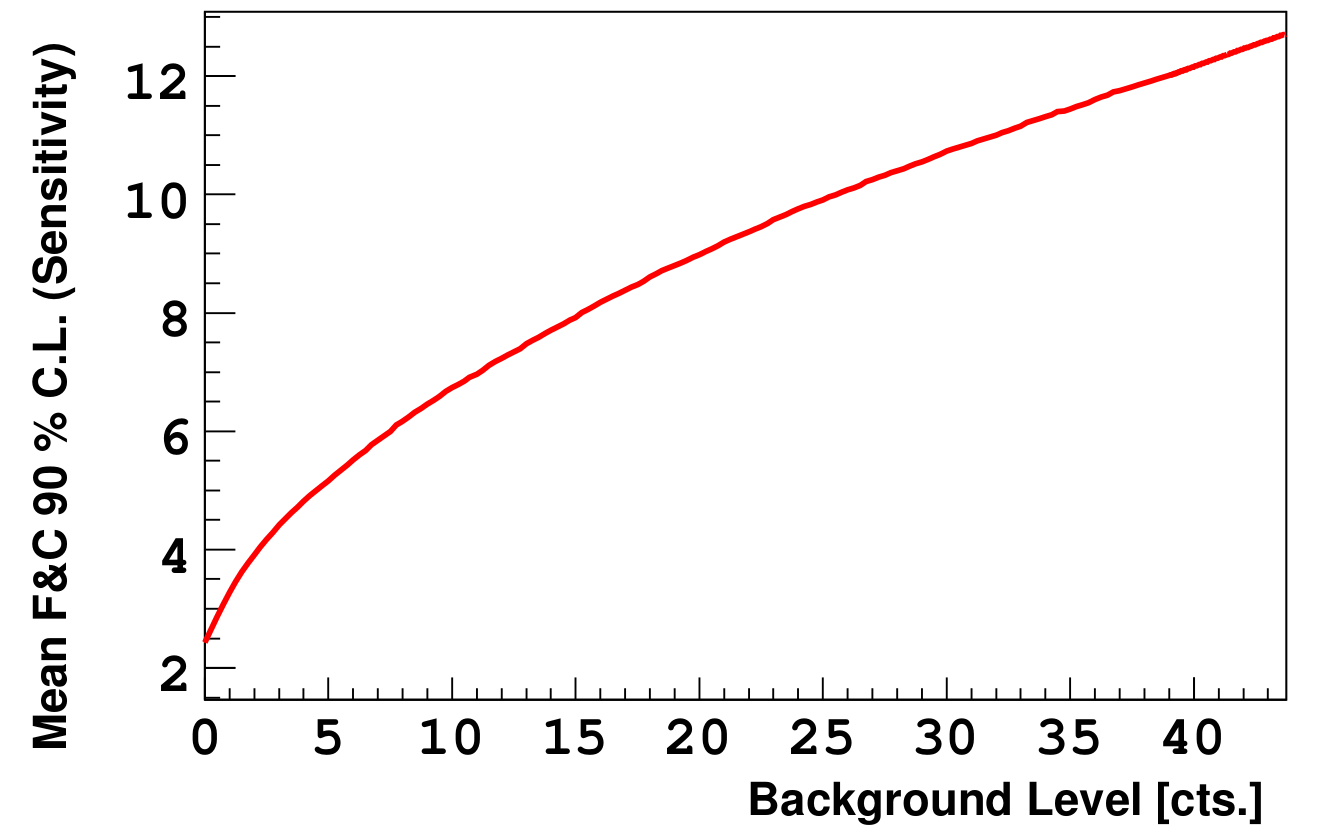
\includegraphics[scale=0.3]{pictures/Chap4/FeldmanAndCousin.png}
\label{FeldmanAndCousin.png}
\caption{aaa}
\end{figure}


\begin{figure}[h!]
\centering
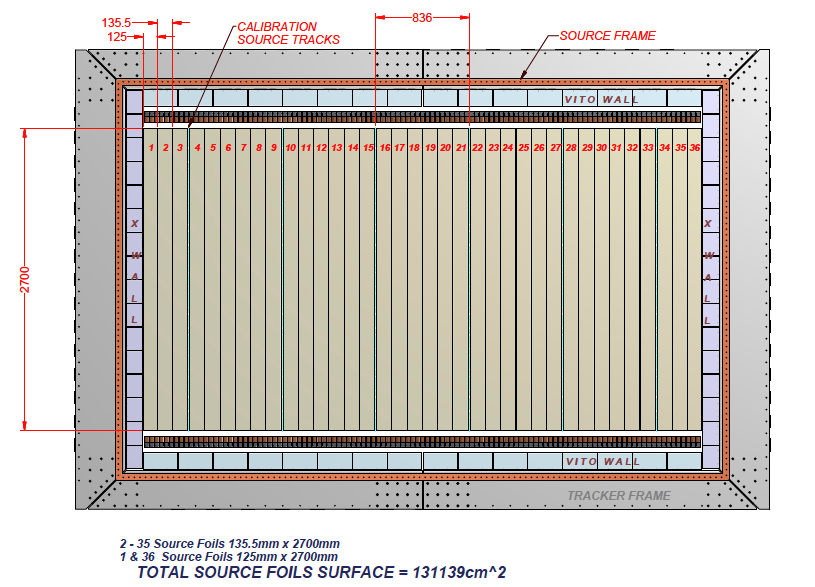
\includegraphics[scale=0.3]{pictures/Chap4/foil.png}
\label{foil.png}
\caption{aaa}
\end{figure}


\begin{figure}[h!]
\centering
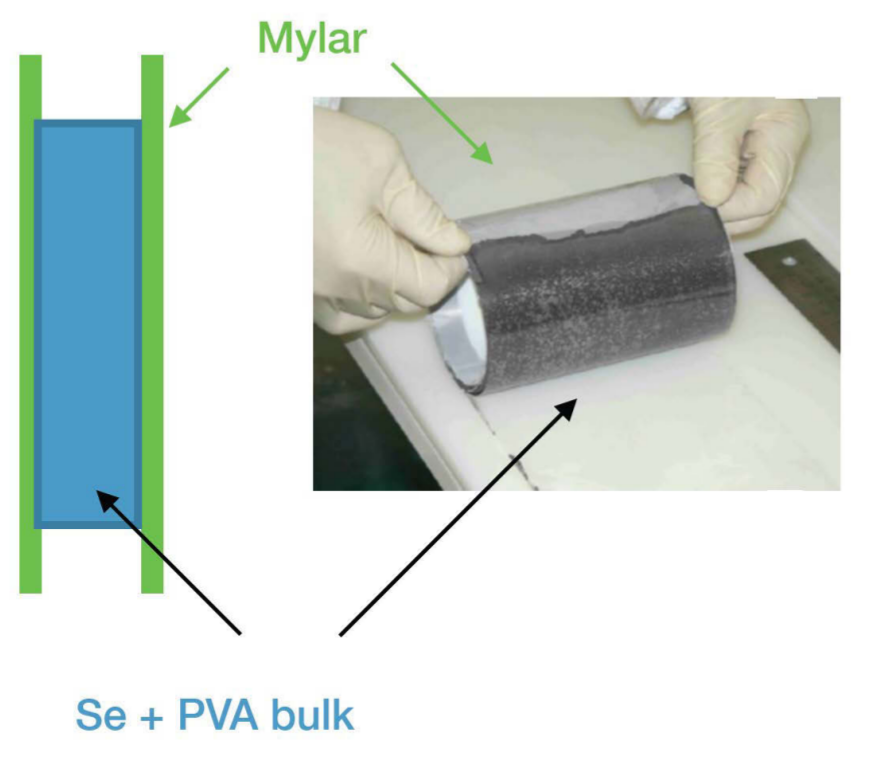
\includegraphics[scale=0.3]{pictures/Chap4/MylarDesign.png}
\label{MylarDesign.png}
\caption{aaa}
\end{figure}


\begin{figure}[h!]
\centering
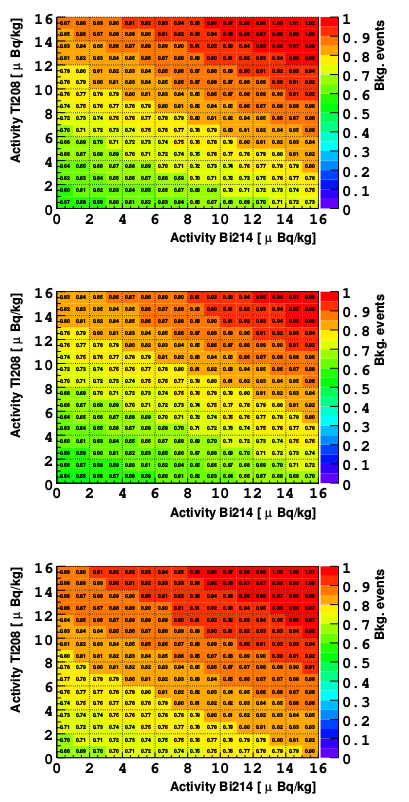
\includegraphics[scale=0.3]{pictures/Chap4/Nbkg_3designs.png}
\label{Nbkg_3designs.png}
\caption{aaa}
\end{figure}


\begin{figure}[h!]
\centering
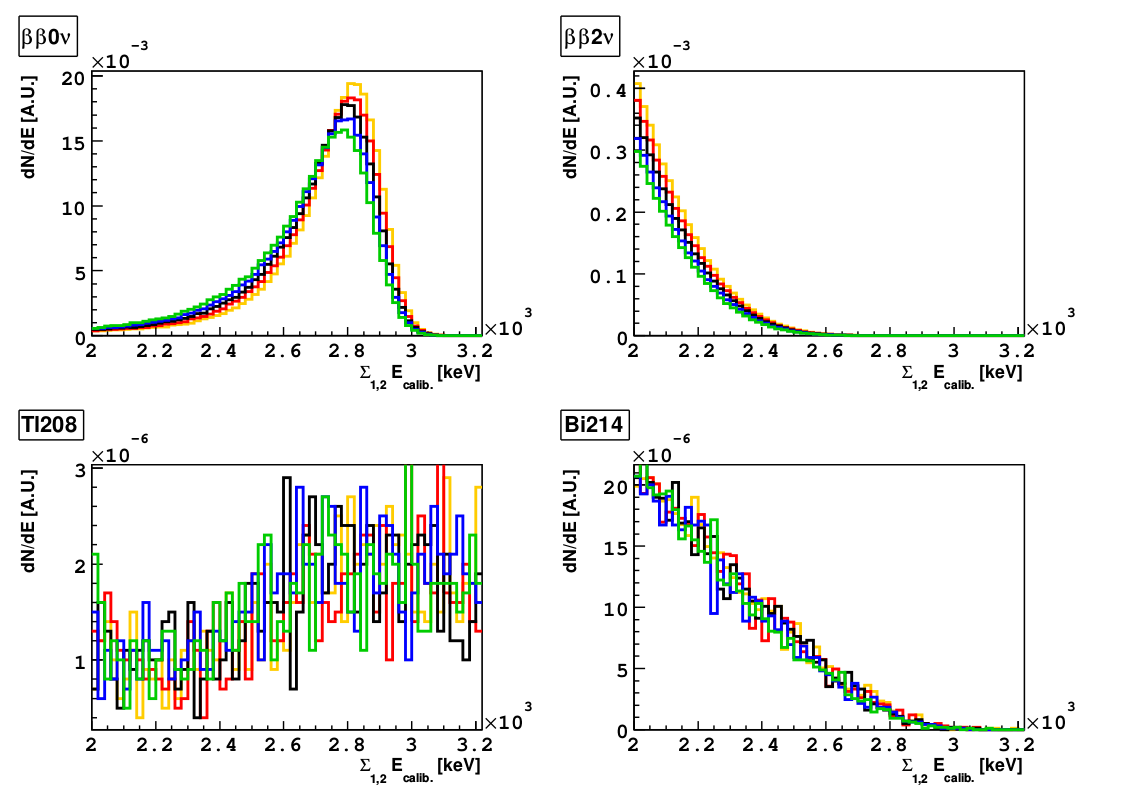
\includegraphics[scale=0.3]{pictures/Chap4/PVAspectra.png}
\label{PVAspectra.png}
\caption{aaa}
\end{figure}


\begin{figure}[h!]
\centering
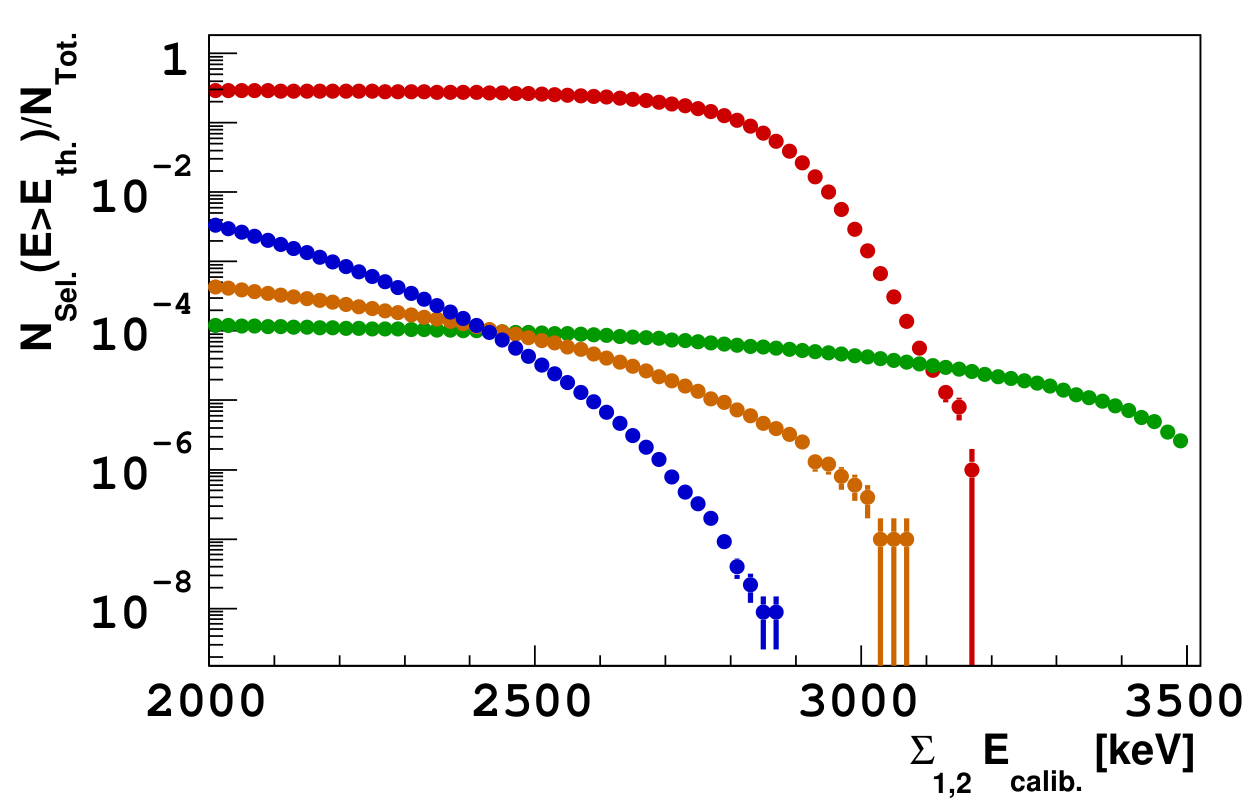
\includegraphics[scale=0.3]{pictures/Chap4/SelectionEfficiency.png}
\label{SelectionEfficiency.png}
\caption{aaa}
\end{figure}


\begin{figure}[h!]
\centering
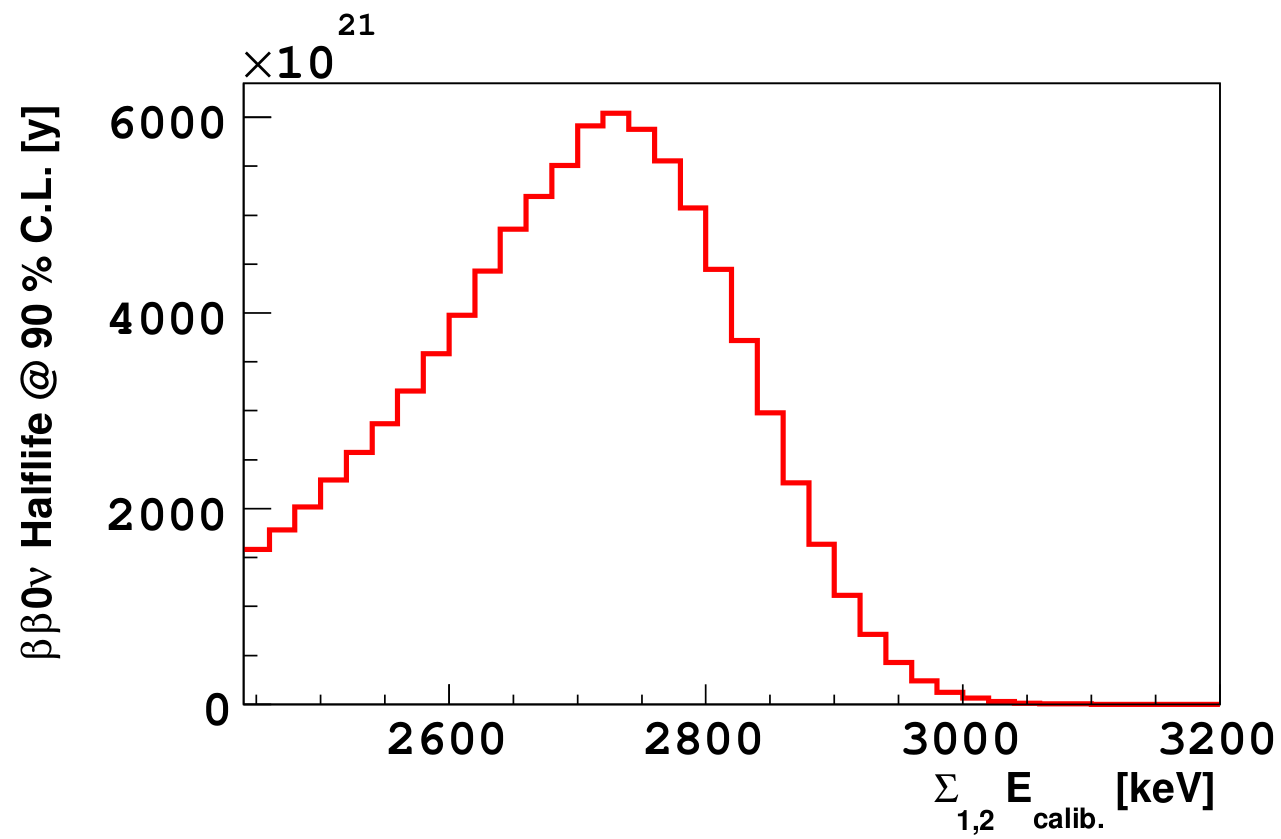
\includegraphics[scale=0.3]{pictures/Chap4/Sens0nu1D.png}
\label{Sens0nu1D.png}
\caption{aaa}
\end{figure}


\begin{figure}[h!]
\centering
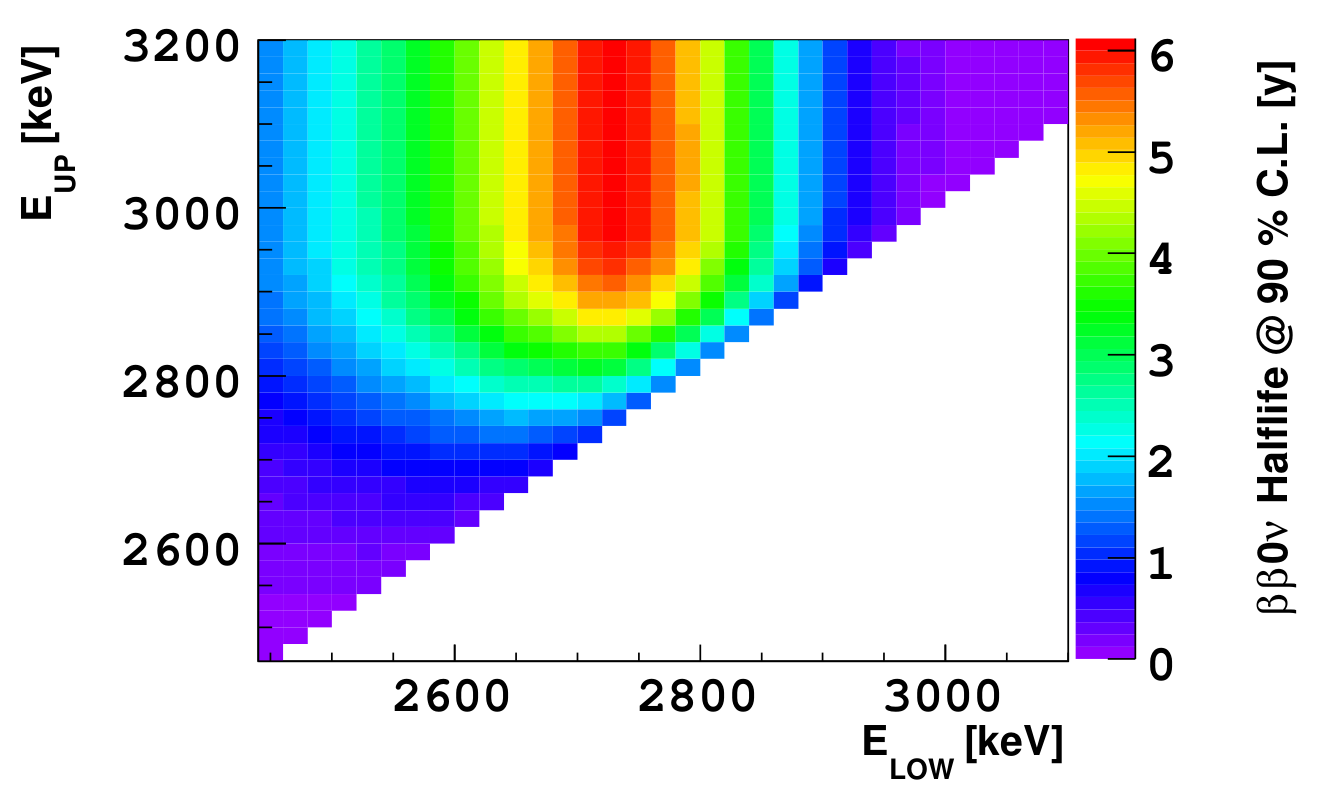
\includegraphics[scale=0.3]{pictures/Chap4/Sens0nu2D.png}
\label{Sens0nu2D.png}
\caption{aaa}
\end{figure}


\begin{figure}[h!]
\centering
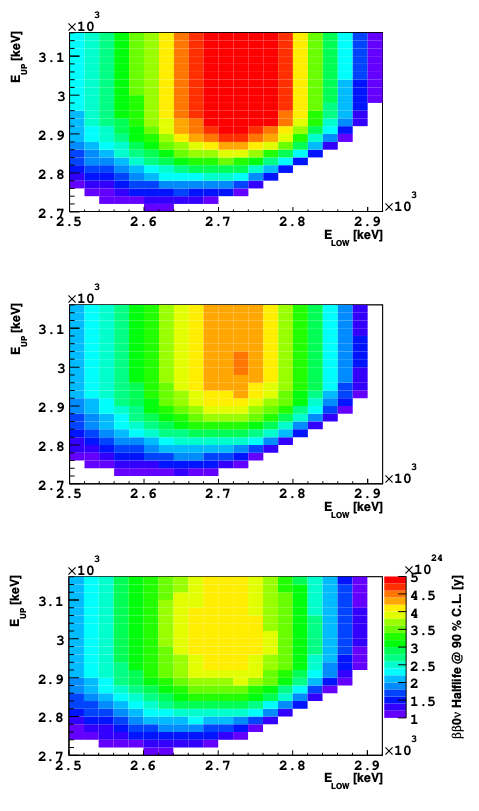
\includegraphics[scale=0.3]{pictures/Chap4/Sens2D-3designs.png}
\label{Sens2D-3designs.png}
\caption{aaa}
\end{figure}


\begin{figure}[h!]
\centering
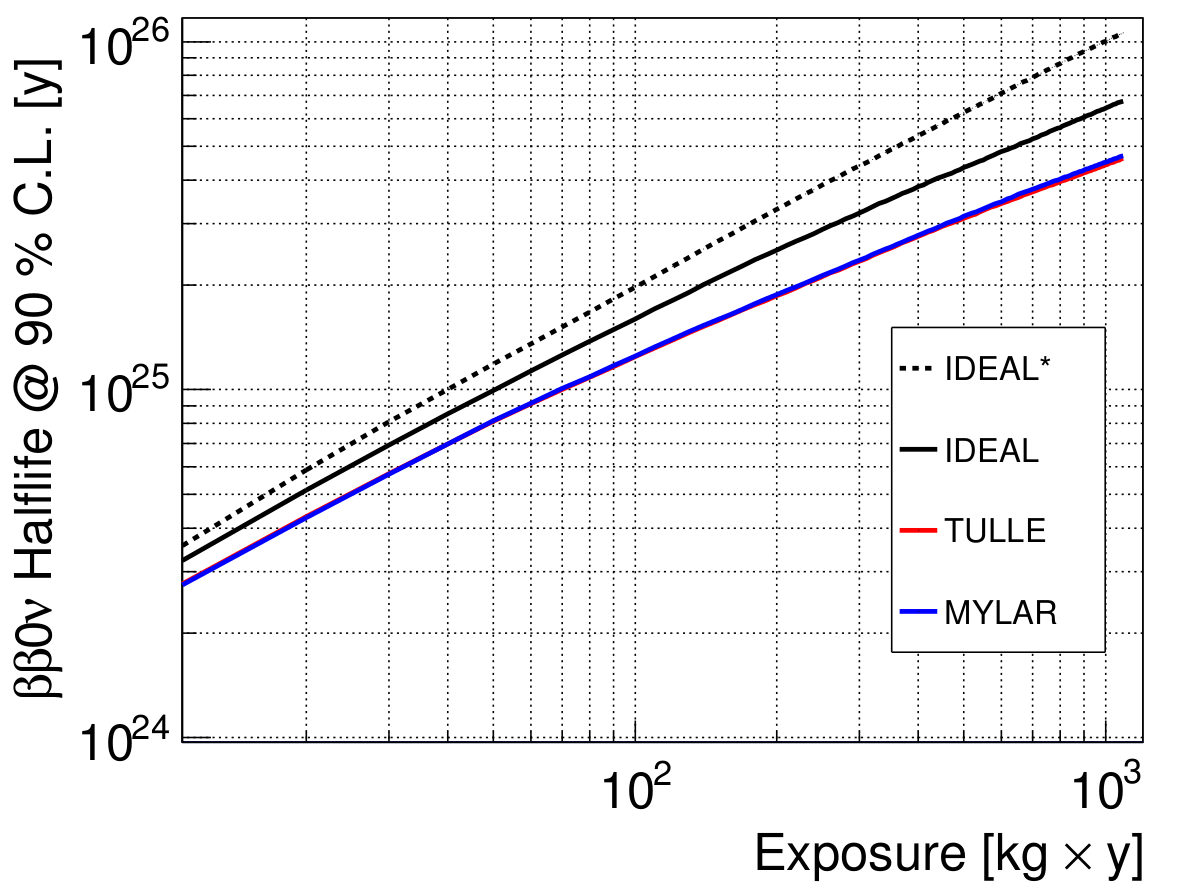
\includegraphics[scale=0.3]{pictures/Chap4/SensVsExposure3Designs.png}
\label{SensVsExposure3Designs.png}
\caption{aaa}
\end{figure}


\begin{figure}[h!]
\centering
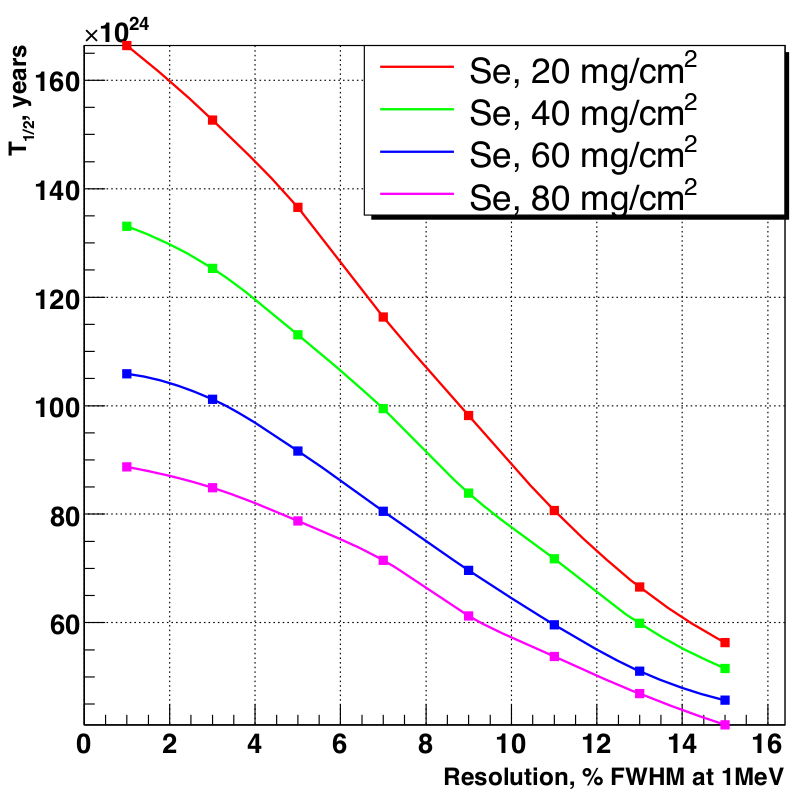
\includegraphics[scale=0.3]{pictures/Chap4/SensVsResolution.png}
\label{SensVsResolution.png}
\caption{aaa}
\end{figure}


\begin{figure}[h!]
\centering
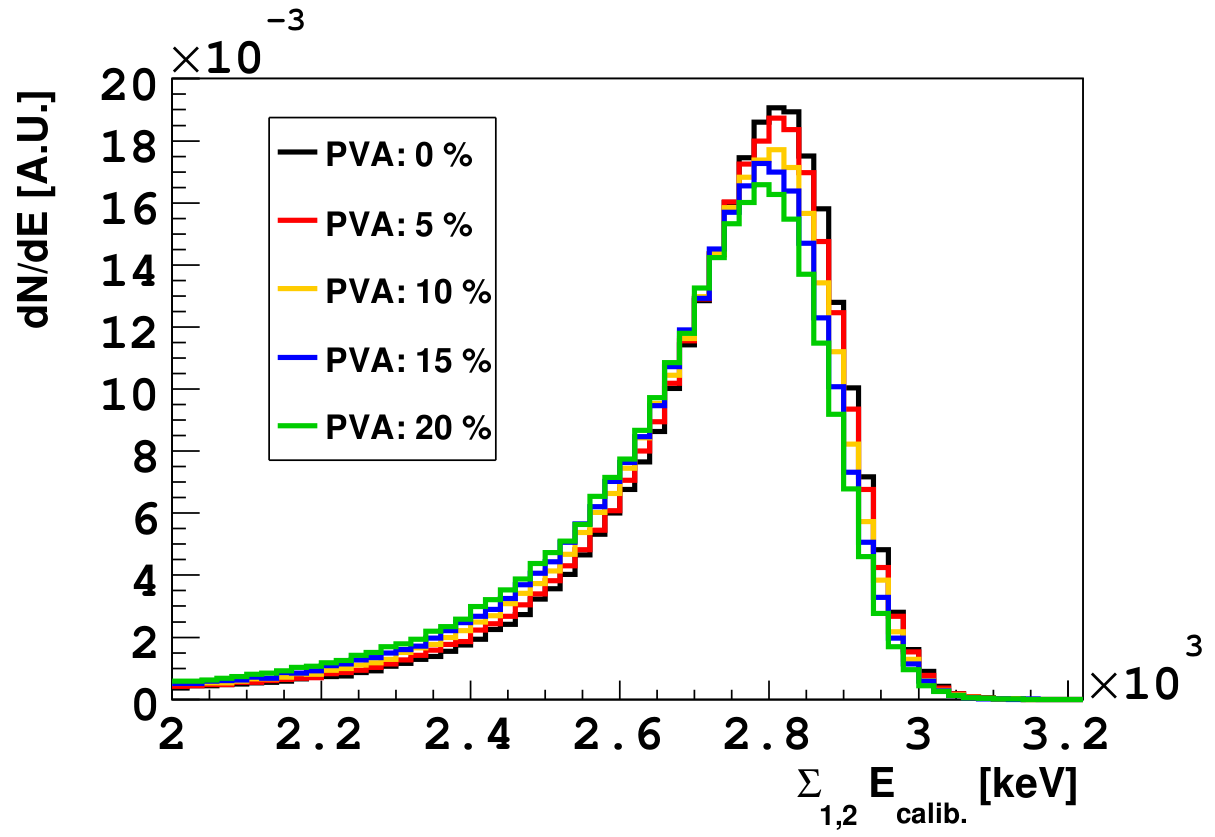
\includegraphics[scale=0.3]{pictures/Chap4/SpectrumPVA.png}
\label{SpectrumPVA.png}
\caption{aaa}
\end{figure}


\begin{figure}[h!]
\centering
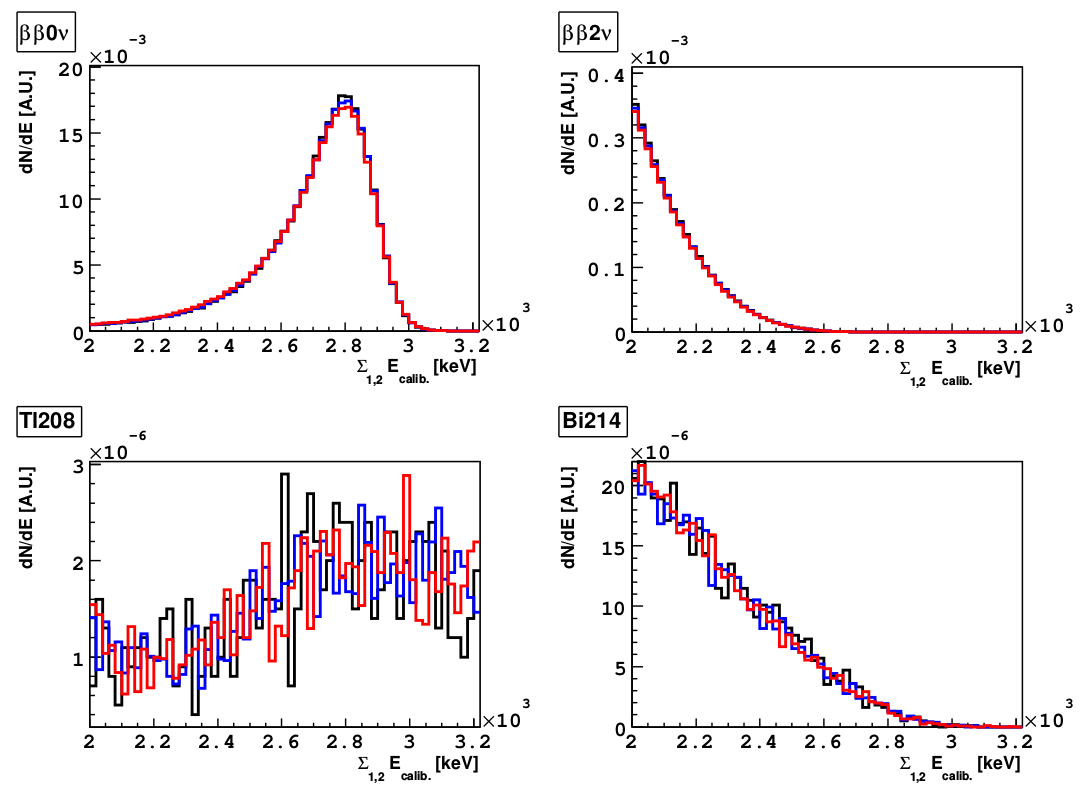
\includegraphics[scale=0.3]{pictures/Chap4/SpectrumThickness.png}
\label{SpectrumThickness.png}
\caption{aaa}
\end{figure}


\begin{figure}[h!]
\centering
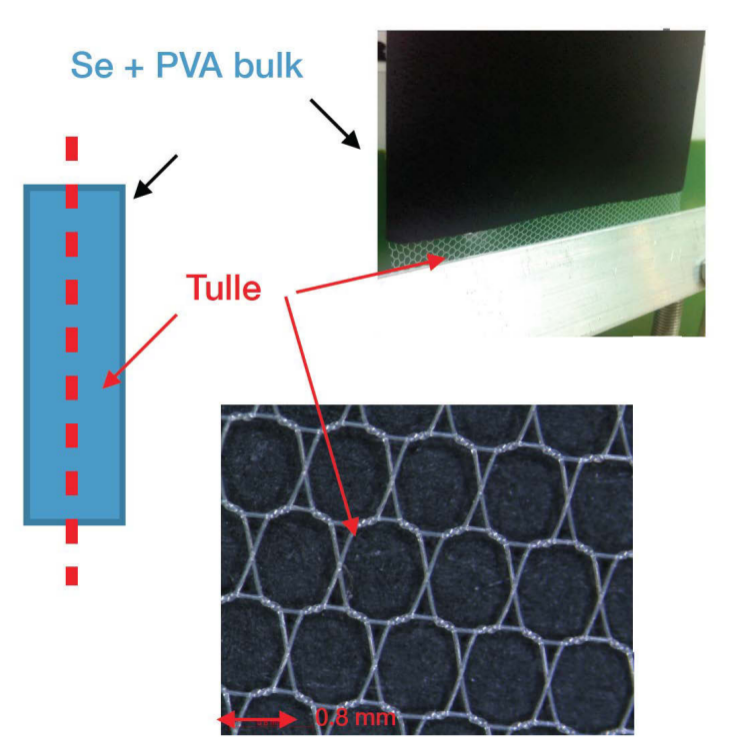
\includegraphics[scale=0.3]{pictures/Chap4/TulleDesign.png}
\label{TulleDesign.png}
\caption{aaa}
\end{figure}

\end{document}
